\section{Cloud computing} 

\subsection{Definition} 
\begin{frame}
	\frametitle{Cloud computing}
	Cloud computing has been defined by the U.S. National
	Institute of Standards and Technology (NIST) as
	"...a model for enabling ubiquitous, convenient, on-demand
	network access to a shared pool of configurable computing
	resources (e.g., networks, servers, storage, applications,
	and services) that can be rapidly provisioned and released
	with minimal management effort or service provider interaction."
\end{frame}

\subsection{Characteristics}
\begin{frame}
	\frametitle{Cloud computing characteristics}
		Cloud computing has several essential characteristics:
	\begin{itemize}
		\item Self-service: Allows cloud consumers to provision instances with computing resources.
		\item Global network access: Access the applications on the instance from the Internet.
		\item Multitenancy: Allows multiple cloud consumers to share the underlying hardware.
		\item Elasticity: Scales out (or scales in) instances to satisfy demand.
		\item Telemetry: Resources can be monitored and metered by the service provider as well as the cloud consumer.
	\end{itemize}
\end{frame}

\subsection{Categories}
\begin{frame}
	\frametitle{Infra service levels}
	\begin{figure}
		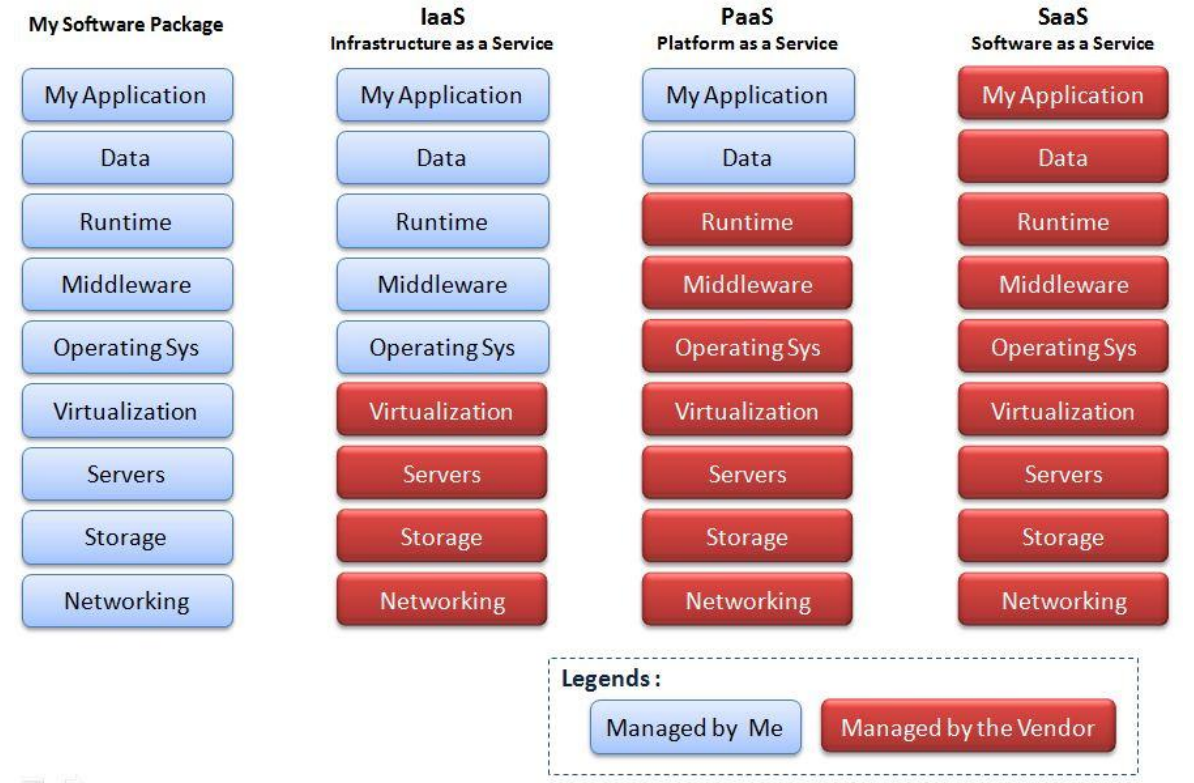
\includegraphics[width=0.8\linewidth]{images/services_cats.png}
	\end{figure}
\end{frame}